\chapter{Results and Discussions}\label{ch:results}
This chapter is organized as follows: Section \ref{sec:ch4_desc_stat} will discuss the results of the descriptive statistics; Section \ref{sec:ch4_morphological_analysis} will discuss the results on the morphological analyses; Section \ref{sec:ch4_structural_analysis} will discuss the structural analyses including the Mathematical structures of the Qur'\=an; Section \ref{sec:ch4_topic_modeling_result} will discuss the results for thematic analyses using both statistical and Large Language models; and finally, 
Section \ref{sec:ch4_relating_islamic_texts} will discuss the use of other Islamic texts that will help in adding more contexts for the Large Language models.
\section{Descriptive Statistics}\label{sec:ch4_desc_stat}
This section will focus on the results of the descriptive statistics of the Qur'\=an's \arb[trans]{ayAt} \arb{ayAt} (verses) and \arb[trans]{kalimat} \arb{kalimAt} or words. Figure \ref{fig:ch4_ayah_word_count} visualizes the frequency of the \arb[trans]{ayAt} \arb{ayAt} and words of the Qur'\=an using a combinations of bar, density, and box plots. The figure is divided into three main parts. The first part is the statistics of the \arb[trans]{ayAt}'s \arb{ayAt} count. It can be seen that in terms of the number of verses, it is generally decreasing just like what the Muslims observed. Table \ref{tbl:desc_stats} summarizes the necessary statistics of Figure \ref{fig:ch4_ayah_word_count}. From the said table, there are 39 \arb[trans]{ayAt} \arb{ayAt} to expect based on the median statistics, and there are about 55 \arb[trans]{ayAt} \arb{ayAt} to expect per \textit{s\=urah} \arb{sUraT} based on the mean statistics. The reason the mean is higher than the median follows from the fact that there are surahs that can be considered outlier because of the large number of \arb[trans]{ayAt} \arb{ayAt}. The annotation on the \textit{s\=urah} \arb{sUraT} with the highest number of \arb[trans]{ayAt} \arb{ayAt} are indicated in Figure \ref{fig:ch4_ayah_word_count}. These \textit{s\=urah} \arb{sUraT} pushes the mean to higher number than the median. Indeed, these \textit{s\=urahs} \arb{sUr} have stretched the shape of the density and the box plots to higher values, suggesting that the data points are more varied. The width of the density and the box plots is measured by the variance and the standard deviation, which is simply the square root of the variance. 

\begin{table}
    \caption{Descriptive statistics of the \arb[trans]{ayAt} \arb{ayAt} counts and the counts of its words}
    \label{tbl:desc_stats}
    \begin{tabularx}{\textwidth}[!h]{XXXX}
        \toprule
        Count Data&Mean&Median&Std. Deviation\\
        \midrule
        Ayahs&54.70&39&53.21\\
        Words&679.20&344&931.18\\
        Words per Ayah&10.27&8.23&6.35\\
        \bottomrule
    \end{tabularx}
\end{table}


\begin{figure}[!t]
    \centering
    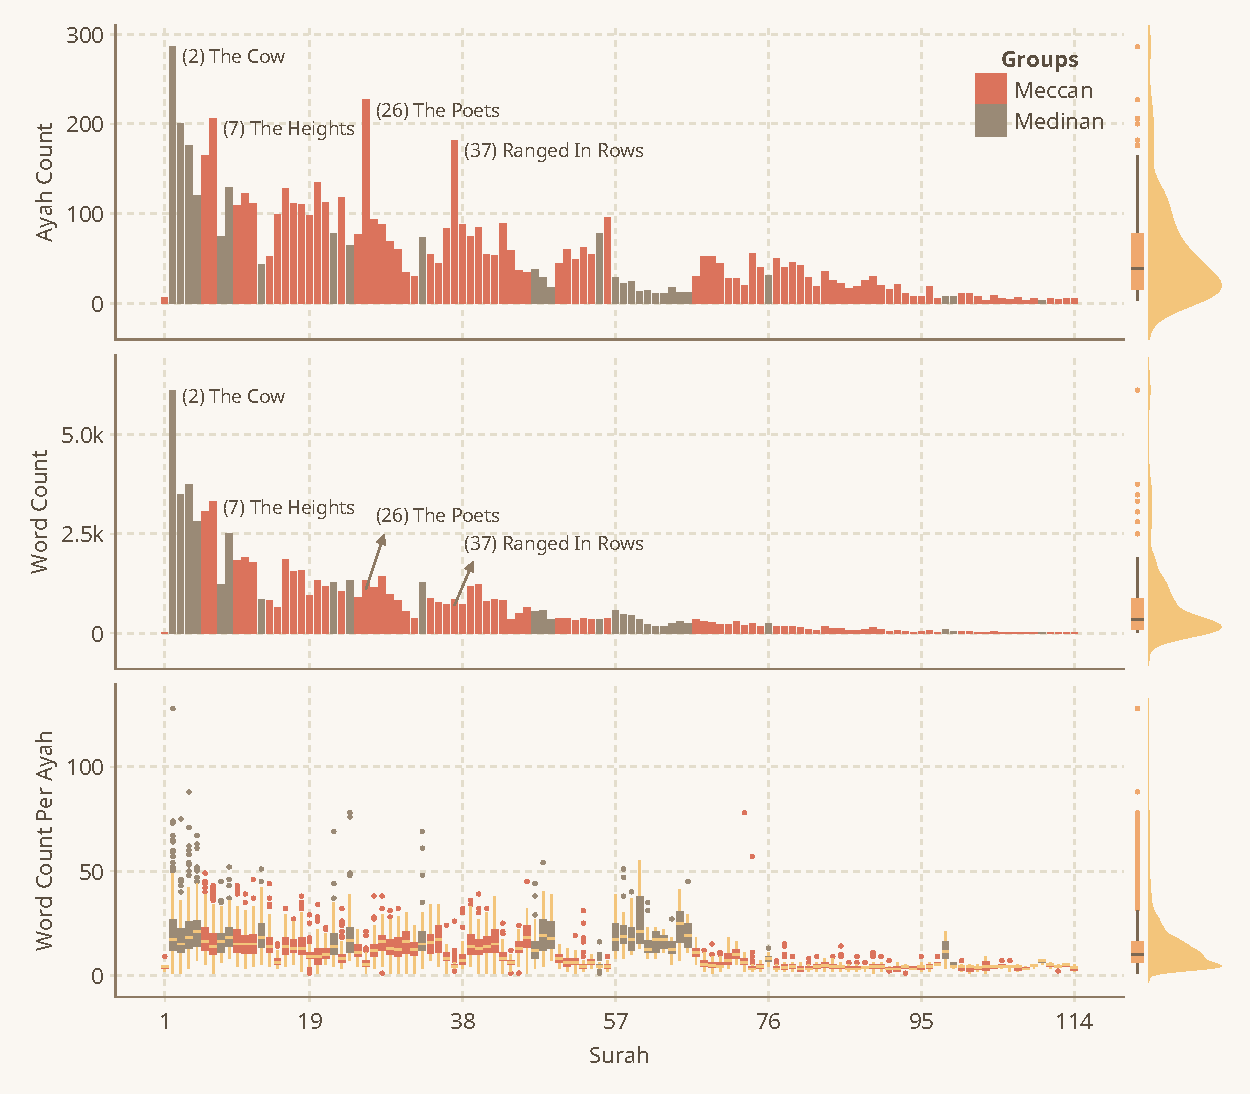
\includegraphics[width=\textwidth]{img/plot1.pdf}
    \caption{Statistics of the words and \arb[trans]{ayAt} \arb{ayAt} (verses) of the Qur'\=an}
    \label{fig:ch4_ayah_word_count}
\end{figure}

\begin{figure}[!t]
    \centering
    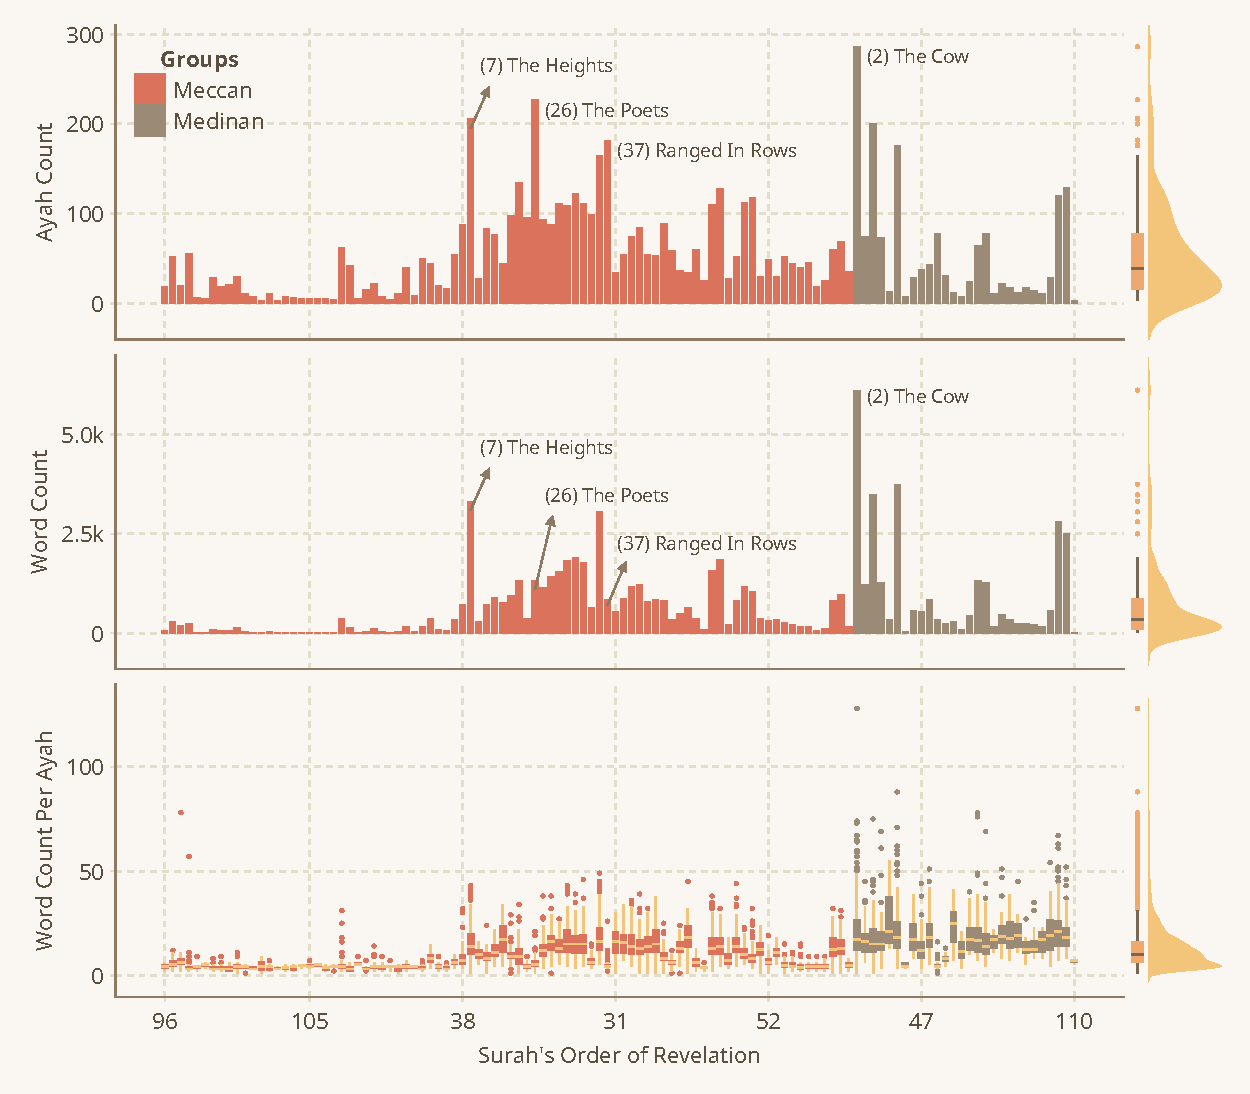
\includegraphics[width=\textwidth]{img/plot2.pdf}
    \caption{Statistics of the words and \arb[trans]{ayAt} \arb{ayAt} (verses) of the Qur'\=an according to revelation order}
    \label{fig:ch4_ayah_word_count_rev_order}
\end{figure}

\subsection{Verses}\label{sec:ch4_desc_stat_verse}
\section{Morphological Analysis}\label{sec:ch4_morphological_analysis}
\section{Structural Analysis}\label{sec:ch4_structural_analysis}
\section{Concentrism Mathematical Formulation}
One of the specific items for the second objective of this paper is on the theory of concentrism, and how can this be formulated statistically, and what are the insights that can be extracted. The idea of the theory of concentrism is that a given texts with define partition follows a ring or concentric structure, which is a literary form where the text is organized in such a way that it mirrors itself around a central point. This means that the beginning and ending sections correspond to each other, moving inward until the center of the text, which often contains the main message or theme. This particular pattern was observed by linguistic experts that it got documented in a book by \citeA{farrin2014structure}. This theory can be defined mathematically as follows:

\begin{defn}[\it Concentric]\label{defn:concentric}
    Let $\mathscr{D}$ be a collection of texts, then $\mathscr{D}$ is said to have a \textit{concentric} or \textit{ring} structure if and only if $\exists\;\mathscr{A}_i\subseteq\mathscr{D},\mathscr{C}\subseteq\mathscr{D},$ and $\mathscr{A}_i^{*}\subseteq\mathscr{D},i\in\mathbb{N}_1$; and that these sets are arranged as follows in $\mathscr{D}$:  $\mathscr{A}_1,\cdots,\mathscr{A}_n,\mathscr{C},\mathscr{A}_1^{*},\cdots,\mathscr{A}_n^{*}$, such that $\mathscr{A}_i^{*}$ \underline{mirrors} $\mathscr{A}_i$ in semantic, and that $\mathscr{C}$ is the center texts of the document $\mathscr{D}$ that is \underline{not related} to both $\mathscr{A}_i$ and $\mathscr{A}_i^{*}$.
\end{defn}

The underlined words above will be used in the next section, because mathematically it begs further definition on what we mean by "mirrors" and "not related" mathematically. This will be defined in the next section. Now, another pattern that was observed by \citeA{farrin2014structure} as chiasmus, which is basically \textit{ring} structure but the second half of the ring after the center is the "complement" or "reversal" of the first half of the document before the center. The following is its mathematical definition.

\begin{defn}[\it Chiasmus]\label{defn:chiasmus}
    Let $\mathscr{D}$ be a collection of texts, then $\mathscr{D}$ is said to have a \textit{concentric} or \textit{ring} structure if and only if $\exists\;\mathscr{A}_i\subseteq\mathscr{D},\mathscr{C}\subseteq\mathscr{D},$ and $\mathscr{A}_i^{*}\subseteq\mathscr{D},i\in\mathbb{N}_{geq 1}$; and that these sets are arranged as follows in $\mathscr{D}$:  $\mathscr{A}_1,\cdots,\mathscr{A}_n,\mathscr{C},\mathscr{A}_1^{c},\cdots,\mathscr{A}_n^{c}$, such that $\mathscr{A}_i^{c}$ is the \underline{complement} or \underline{reversal} of $\mathscr{A}_i$ in semantic, and that $\mathscr{C}$ is the center texts of the document $\mathscr{D}$ that is \underline{not related} to both $\mathscr{A}_i$ and $\mathscr{A}_i^{c}$.
\end{defn}
There are other structures that can be observed in the Qur'\=an, like \textit{parallelism} where themes are repeated in other \arb[trans]{sUraT} \arb{sUraT}; and \textit{segment structure}, where a particular segment starts and ends with similar phrases or themes, creating a bracket around the content; but, these other structures are not studied in this paper. Apart from this, there is also the "mathematical patterns" of the Qur'\=an which has been extensively studied by \citeA{rashad1981}, but this is also not studied in this paper.
\subsection{Bayesian Optimization}\label{sec:bayes-opt}
From Defn. \ref{defn:concentric} and \ref{defn:chiasmus}, it both states that, a document $\mathscr{D}$ may only be considered \textit{concentric} or \textit{chiasmus} if and only if "there exist", denoted by the symbol $\exists$. Indeed, subset of texts $\mathscr{A}_i$s, $\mathscr{C}$, and $\mathscr{A}_i^{*}$ or $\mathscr{A}_i^{\text{c}}$ are all determined manually by the investigator. In this study, we propose to automate the determination of these subsets of texts of document $\mathscr{D}$, and this is through the use of an optimization algorithm called Bayesian Optimization. The idea behind Bayesian optimization is that it approximates the objective function with a \textit{surrogate} function, and using this surrogate to find the global maximum or minimum of the objective function. Furthermore, it does this by fitting the surrogate function to the objective function in as few input points or iteration as possible. As such, an \textit{acquisition} function is needed for choosing smartly the next input points to be used for fitting the surrogate. Using these components, a Bayes' Theorem is used in fitting the surrogate.

To do this, a \textit{global objective function} must be defined, for this study, the cosine similarity discussed in the previous section will be used as the said cost function that will either be maximized or minimized. The core model for this optimization is the Gaussian Process defined below.
\subsubsection{Surrogate Function}
The surrogate function aims to approximate the objective function. In Bayesian, optimization, the surrogate function is defined by the Gaussian process (GP).
\begin{defn}[\it Gaussian Process]\label{defn:gp}
    Let $Y_1,Y_2,\cdots,Y_T$ be sequence of random variables such that $Y_t\in\mathbf{Y}$, then the sequence is a \textit{Gaussian process} (GP) if and only if $\mathbf{Y}\overset{\mathrm{iid}}{\sim}\mathcal{N}(\boldsymbol{\mu}, \boldsymbol{\Sigma})$.
\end{defn}
\begin{defn}[\it Parameter Space]\label{defn:parameter_space}
    Let $\mathbf{s}_i\in\mathscr{D}$ be a word embedding of an \arb[trans]{'ayaT} \arb{'ayaT} in document $\mathscr{D}$, which can be a \arb[trans]{sUraT} \arb{sUraT}, group of \arb[trans]{suwar} \arb{suwar}, or group of \arb[trans]{'Ayat} \arb{'Ayat} within a \arb[trans]{sUraT} \arb{sUraT}. Further, suppose $\mathscr{A}_i,\mathscr{C},\mathscr{A}_i^{*}\subseteq\mathscr{D}$ such that $\mathscr{A}_i:=\{\mathbf{s}_{i,1},\cdots,\mathbf{s}_{i,n}\},\linebreak\mathscr{C}:=\{\mathbf{s}_{n+1},\cdots,\mathbf{s}_{n+c}\}$, and $\mathscr{A}_i^{*}:=\{\mathbf{s}_{i,(n+c+1)},\cdots,\mathbf{s}_{i,(n+c+n)}\}$, then the \textit{parameters} to be optimized are assigned to $\mathbf{v}:=[n,c]^{\text{T}}$, and since $n,c,m\in\mathbb{N}_{\geq 2}$, then the \textit{parameter space} is $\mathscr{P}:=\mathbb{N}_{\geq 2}\times\mathbb{N}_{\geq 2}\times\mathbb{N}_{\geq 2}=(\mathbb{N}_{\geq 2})^3$, so that $\mathbf{v}\in\mathscr{P}$. 
\end{defn}
\begin{defn}[\it Semi-Circle Cost Function]\label{defn:semi_circle_cost}
    From Defn. \ref{defn:parameter_space}, let $r_1$ to denote that $\mathscr{A}_i$ is "related" to $\mathscr{A}_i^{*}$, and $r_2$ to denote that $\mathscr{A}_i$ is "reversal" of $\mathscr{A}_i^{*}$, such that $\eta:=\{r_1,r_2\}$, then  the \textit{semi-circle} cost function between $\mathscr{A}_i$ and $\mathscr{A}_i^{*}$ is defined as:
    \begin{equation}
        \operatorname{\gamma}_{a}(\mathbf{v};\mathscr{A}_i,\mathscr{A}_i^{*},\eta):=\begin{cases}
            \frac{1}{n}\sum_{k=1}^{n}\cos\left(\theta_{\mathbf{s}_{i,k};\mathbf{s}_{i,n+l}}\right),&\text{if}\;\eta=r_1\\
            1-\frac{1}{n}\sum_{k=1}^{n}\cos\left(\theta_{\mathbf{s}_{i,k};\mathbf{s}_{i,n+l}}\right),&\text{if}\;\eta=r_2\\
        \end{cases}
    \end{equation}
\end{defn}
\begin{defn}[\it Center Cost Function]\label{defn:center_cost}
    From Defn. \ref{defn:parameter_space}, the \textit{center} cost function is defined as:
    \begin{equation}
        \operatorname{\gamma}_{b}(\mathbf{v};\mathscr{A}_i,\mathscr{C},\mathscr{A}_i^{*}):=2-\frac{1}{nc}\sum_{k=1}^{n}\sum_{l=1}^{c}\cos\left(\theta_{\mathbf{s}_{i,k};\mathbf{s}_{n+l}}\right)-\frac{1}{nc}\sum_{k=1}^{n}\sum_{l=1}^{c}\cos\left(\theta_{\mathbf{s}_{n+l};\mathbf{s}_{i,n+c+k}^{*}}\right).
    \end{equation}
\end{defn}
\begin{defn}[\it Global Cost Function]\label{defn:global_cost}
    From Defn. \ref{defn:parameter_space}-\ref{defn:center_cost}, the \textit{global} cost function is defined as:
    \begin{equation}
        \operatorname{\gamma}_{g}(\mathbf{v};\mathscr{A}_i,\mathscr{C},\mathscr{A}_i^{*},\eta):=\operatorname{\gamma}_{a}(\mathbf{v};\mathscr{A}_i,\mathscr{A}_i^{*},\eta)+\operatorname{\gamma}_{b}(\mathbf{v};\mathscr{A}_i,\mathscr{C},\mathscr{A}_i^{*})
    \end{equation}
\end{defn}
\begin{defn}[\it Optimal Parameters] From Defn. \ref{defn:global_cost}, the optimal parameters would be:
\begin{equation}
    \hat{\mathbf{v}}:=\underset{n,c}{\arg\min}\operatorname{\gamma}_{g}(\mathbf{v};\mathscr{A}_i,\mathscr{C},\mathscr{A}_i^{*},\eta),
\end{equation}    
\end{defn}
\begin{prop}\label{prop:hypedist}
    Let $\mathscr{P}$ be the parameter space and suppose $\gamma(\mathbf{v})\overset{\mathrm{iid}}{\sim}\mathcal{N}(m(\mathbf{v}),k(\mathbf{v},\mathbf{v})), \linebreak\forall \mathbf{v}\in\mathscr{P}$, then for any $\boldsymbol{\delta}:=[\gamma(\mathbf{v}_1),\cdots,\gamma(\mathbf{v}_n)]^{\top}$, $\boldsymbol{\delta}\overset{\mathrm{iid}}{\sim}\mathcal{N}_n(\mathbf{m},\mathbf{K})$, where 
    \begin{equation}
        \mathbf{m}:=[m(\mathbf{v}_1),\cdots,m(\mathbf{v}_n)]^{\top}
    \end{equation}
    and
    \begin{equation}
        \mathbf{K}:=\left[\begin{matrix}
        k(\mathbf{v}_1,\mathbf{v}_1)&\cdots&k(\mathbf{v}_1,\mathbf{v}_n)\\
        \vdots&\ddots&\vdots\\
        k(\mathbf{v}_n,\mathbf{v}_1)&\cdots&k(\mathbf{v}_n,\mathbf{v}_n)\\
        \end{matrix}\right]
    \end{equation}
\end{prop}
\begin{proof}
    The proof follows from the proof of Theorem 1.2.9 of \citeA{muirhead2005}.
\end{proof}
\begin{remark}
    From Proposition \ref{prop:hypedist} and Definition \ref{defn:gp}, $\boldsymbol{\delta}$ is a GP.
\end{remark}
\begin{prop}\label{prop:jointpdf}
    From Proposition \ref{prop:hypedist}, suppose $\boldsymbol{\delta}_{*}:=[\gamma(\mathbf{v}_{n+1}),\cdots,\gamma(\mathbf{v}_{n+p})]^{\top}$, such that $\boldsymbol{\delta}_{*}\overset{\mathrm{iid}}{\sim}\mathcal{N}_p(\mathbf{m}_*,\mathbf{K}_*)$ then 
    \begin{equation}
        \left[
        \begin{matrix}
            \boldsymbol{\delta}\\
            \boldsymbol{\delta}_{*}\\
        \end{matrix}
        \right]\overset{\mathrm{iid}}{\sim}
        \mathcal{N}_{n+p}\left(\left[
        \begin{matrix}
            \mathbf{m}\\
            \mathbf{m}_{*}\\
        \end{matrix}
        \right],\left[
        \begin{matrix}
            \mathbf{K}&\mathbf{K}_{*}\\
            \mathbf{K}_{*}^{\top}&\mathbf{K}_{**}\\
        \end{matrix}
        \right]\right)
    \end{equation}
\end{prop}
\begin{proof}
    Let $\mathbf{u}:=[\boldsymbol{\delta},\boldsymbol{\delta}_{*}]^{\top}$, then $\mathbf{u}=[\gamma(\mathbf{v}_1),\cdots,\gamma(\mathbf{v}_{n+p})]^{\top}$. Further, since $\mathbf{\gamma}(\mathbf{v}_i)\overset{\mathrm{iid}}{\sim}\mathcal{N}(m(\mathbf{v}_i),k(\mathbf{v}_i,\mathbf{v}_i)),\forall i\in\mathbb{N}_{\leq n+p}$, then the joint distribution of the $\gamma(\mathbf{v}_i)$s, i.e. $\mathrm{Pr}(\mathbf{u})$, follows from the proof of Theorem 1.2.9 of \citeA{muirhead2005}.
\end{proof}
\begin{cor}\label{cor:condpdf}
From Proposition \ref{prop:jointpdf}, let $\mathbf{m}$ and $\mathbf{m}_{*}$ be zero vectors, then the following conditional distribution is true:
    \begin{equation}\label{eq:gp_updater}    \boldsymbol{\delta}_*\mid\boldsymbol{\delta}\overset{\mathrm{iid}}{\sim}\mathcal{N}_{p}(\mathbf{K}_{*}^{\top}\mathbf{K}^{-1}\boldsymbol{\delta},\mathbf{K}_{**}-\mathbf{K}_{*}^{\top}\mathbf{K}^{-1}\mathbf{K}_{*}).
\end{equation}
\end{cor}
\begin{proof}
    The proof follows by reversing the condition from $\mathbf{X}_1\mid\mathbf{X}_2$ to $\mathbf{X}_2\mid\mathbf{X}_1$ of the proof of Theorem 1.2.11 of \cite{muirhead2005}.
\end{proof}
\begin{defn}[\it Lower Confidence Bound]\label{defn:lcb}
    Let $m(\mathbf{v})$ be the mean of the GP, then the Lower Confidence Bound (LCB) notated as $\xi$ is given by
    \begin{equation}
        \xi(\mathbf{v}\mid\zeta):=m(\mathbf{v})-\zeta k(\mathbf{v},\mathbf{v}),
    \end{equation}
    where $\zeta$ is the balancing factor.
\end{defn}
The \textit{global cost} computed from the global cost function in Defn. \ref{defn:global_cost} is approximated by the Gaussian process (the surrogate function) defined in Defn. \ref{defn:gp} through Proposition \ref{prop:hypedist}. So that, for any new observed global cost computed from the new parameter input $\mathbf{v}$, chosen by the acquisition function defined in Defn. \ref{defn:lcb}, the joint distribution with the previous global cost is given in Proposition \ref{prop:jointpdf}. Therefore, computing for the conditional distribution of the new global costs conditioned on previous global cost is given in Corollary \ref{cor:condpdf}. The process of acquiring new parameter candidate and computing the global cost is done iteratively. The algorithm converges until there is no significant changes on the new parameter candidate relative to the preceding parameter candidate, or alternatively, until a specified maximum iteration.
\begin{center}
    \textcolor{red}{add theoretical Bayes theorem computations here}
\end{center}
\subsection{Discussions on Islamic Philosophy of Qur'\=an's Structural Analysis}
\newpage
\section{Topic Modeling}\label{sec:ch4_topic_modeling_result}
\subsection{Latent Dirichlet Allocation}
\subsection{Bidirectional Encoder Representation from Transformer}
\subsection{Generative Pre-Trained Transformer}
\section{Relating to other Islamic Texts and Analyses}\label{sec:ch4_relating_islamic_texts}
\subsection{Retrieval-Augmented Generation Approach}
\section{Limitations of the Models}